\documentclass[nooutcomes]{ximera}
%\documentclass[space,handout,nooutcomes]{ximera}

% For preamble materials

\usepackage{pgf,tikz}
\usepackage{mathrsfs}
\usetikzlibrary{arrows}
\usepackage{framed}
\usepackage{amsmath}
\pgfplotsset{compat=1.17}

\def\fixnote#1{\begin{framed}{\textcolor{red}{Fix note: #1}}\end{framed}}  % Allows insertion of red notes about needed edits
%\def\fixnote#1{}

\def\detail#1{{\textcolor{blue}{Detail: #1}}}   

\pdfOnly{\renewenvironment{image}[1][]{\begin{center}}{\end{center}}}

\graphicspath{
  {./}
  {chapter1/}
  {chapter2/}
  {chapter4/}
  {proofs/}
  {graphics/}
  {../graphics/}
}

\newenvironment{sectionOutcomes}{}{}


%%% This set of code is all of our user defined commands
\newcommand{\bysame}{\mbox{\rule{3em}{.4pt}}\,}
\newcommand{\N}{\mathbb N}
\newcommand{\C}{\mathbb C}
\newcommand{\W}{\mathbb W}
\newcommand{\Z}{\mathbb Z}
\newcommand{\Q}{\mathbb Q}
\newcommand{\R}{\mathbb R}
\newcommand{\A}{\mathbb A}
\newcommand{\D}{\mathcal D}
\newcommand{\F}{\mathcal F}
\newcommand{\ph}{\varphi}
\newcommand{\ep}{\varepsilon}
\newcommand{\aph}{\alpha}
\newcommand{\QM}{\begin{center}{\huge\textbf{?}}\end{center}}

\renewcommand{\le}{\leqslant}
\renewcommand{\ge}{\geqslant}
\renewcommand{\a}{\wedge}
\renewcommand{\v}{\vee}
\renewcommand{\l}{\ell}
\newcommand{\mat}{\mathsf}
\renewcommand{\vec}{\mathbf}
\renewcommand{\subset}{\subseteq}
\renewcommand{\supset}{\supseteq}
%\renewcommand{\emptyset}{\varnothing}
%\newcommand{\xto}{\xrightarrow}
%\renewcommand{\qedsymbol}{$\blacksquare$}
%\newcommand{\bibname}{References and Further Reading}
%\renewcommand{\bar}{\protect\overline}
%\renewcommand{\hat}{\protect\widehat}
%\renewcommand{\tilde}{\widetilde}
%\newcommand{\tri}{\triangle}
%\newcommand{\minipad}{\vspace{1ex}}
%\newcommand{\leftexp}[2]{{\vphantom{#2}}^{#1}{#2}}

%% More user defined commands
\renewcommand{\epsilon}{\varepsilon}
\renewcommand{\theta}{\vartheta} %% only for kmath
\renewcommand{\l}{\ell}
\renewcommand{\d}{\, d}
\newcommand{\ddx}{\frac{d}{dx}}
\newcommand{\dydx}{\frac{dy}{dx}}


\usepackage{bigstrut}


\title{Quadrilaterals}
\author{Brad Findell}
\begin{document}
\begin{abstract}
Proof. 
\end{abstract}
\maketitle


\begin{problem}
Adapted from Ohio's 2017 Geometry released item 13. 

Two pairs of parallel lines intersect to form a parallelogram as shown.  
\begin{image}
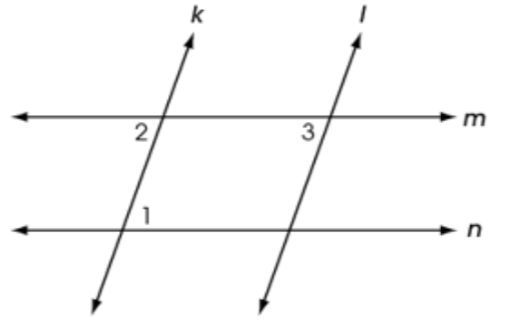
\includegraphics{Q13.png}
\end{image}
Complete the following proof that opposite angles of a parallelogram are congruent: 

\begin{enumerate}
\item $\angle 1 \cong \angle 2$ as \wordChoice{\choice{opposite angles}\choice[correct]{alternate interior angles}\choice{corresponding angles}}
for parallel lines \wordChoice{\choice[correct]{$m$ and $n$}\choice{$k$ and $l$}}.
\item $\angle 3 \cong \angle 2$ as \wordChoice{\choice{opposite angles}\choice{alternate interior angles}\choice[correct]{corresponding angles}}for parallel lines \wordChoice{\choice{$m$ and $n$}\choice[correct]{$k$ and $l$}}.
\item Then $\angle 1 \cong \angle 3$ because they are both congruent 
to $\angle 2$. 
\end{enumerate}
\end{problem}

\begin{problem}
Adapted from Ohio's 2018 Geometry released item 21. 

Given the parallelogram $WXYZ$, prove that $\overline{WX}\cong\overline{YZ}$. 

\begin{image}
\definecolor{qqqqff}{rgb}{0.,0.,1.}
\begin{tikzpicture}[line cap=round,line join=round,>=triangle 45,x=1.0cm,y=1.0cm]
\clip(-2,-0.6) rectangle (6,2.5);
\draw [line width=0.8pt] (0.,0.)-- (4.,0.);
\draw [line width=0.8pt] (4.,0.)-- (5.,2.);
\draw [line width=0.8pt] (5.,2.)-- (1.,2.);
\draw [line width=0.8pt] (1.,2.)-- (0.,0.);
\draw [line width=0.8pt] (1.,2.)-- (4.,0.);
\begin{scriptsize}
\draw [fill=qqqqff] (0.,0.) circle (1.2pt);
\draw[color=qqqqff] (-0.28,-0.03) node {$Z$};
\draw [fill=qqqqff] (1.,2.) circle (1.2pt);
\draw[color=qqqqff] (0.86,2.29) node {$W$};
\draw [fill=qqqqff] (4.,0.) circle (1.2pt);
\draw[color=qqqqff] (4.22,0.07) node {$Y$};
\draw [fill=qqqqff] (5.,2.) circle (1.2pt);
\draw[color=qqqqff] (5.14,2.29) node {$X$};
\end{scriptsize}
\end{tikzpicture}
\end{image}

\fixnote{It really would help to have an online environment that allows students to mark diagrams.}

Complete the proof below: 
\begin{enumerate}
\item $\angle ZWY \cong \angle XYW$ as \wordChoice{\choice[correct]{alternate interior angles}\choice{corresponding angles}\choice{opposite angles}} for parallel segments \wordChoice{\choice[correct]{$\overline{WZ}$ and $\overline{XY}$}\choice{$\overline{WX}$ and $\overline{YZ}$}}.
\item $\angle ZYW \cong \angle XWY$ for the same reason, this time for parallel segments \wordChoice{\choice{$\overline{WZ}$ and $\overline{XY}$}\choice[correct]{$\overline{WX}$ and $\overline{YZ}$}}.
\item $\overline{WY}\cong\overline{YW}$ because a segment is congruent to itself. 
\item $\triangle WYZ \cong \triangle YWX$ by \wordChoice{\choice{SAS}\choice[correct]{ASA}\choice{SSS}}.  
\item Then $\overline{YZ}\cong\overline{WX}$ as corresponding parts of congruent triangles. 
\end{enumerate}
\fixnote{Maybe number the angles.}

\end{problem}

\end{document}
